% Created 2020-04-30 jue 15:59
% Intended LaTeX compiler: pdflatex
\documentclass[presentation,aspectratio=1610]{beamer}
\usepackage[utf8]{inputenc}
\usepackage[T1]{fontenc}
\usepackage{graphicx}
\usepackage{grffile}
\usepackage{longtable}
\usepackage{wrapfig}
\usepackage{rotating}
\usepackage[normalem]{ulem}
\usepackage{amsmath}
\usepackage{textcomp}
\usepackage{amssymb}
\usepackage{capt-of}
\usepackage{hyperref}
\usepackage{khpreamble}
\usepackage{pgfplots}
\usepackage{pdfpages}
\usepgfplotslibrary{groupplots}
\usepackage[american,siunitx]{circuitikz}
\usetikzlibrary{arrows,shapes,calc,positioning}
\usetheme{default}
\author{Kjartan Halvorsen}
\date{\today}
\title{Pneumatic systems}
\hypersetup{
 pdfauthor={Kjartan Halvorsen},
 pdftitle={Pneumatic systems},
 pdfkeywords={},
 pdfsubject={},
 pdfcreator={Emacs 26.3 (Org mode 9.3.6)}, 
 pdflang={English}}
\begin{document}

\maketitle

\section{Intro}
\label{sec:orgd4018e1}
\begin{frame}[label={sec:orgd4c9f5e}]{Pneumatic elements}
\begin{center}
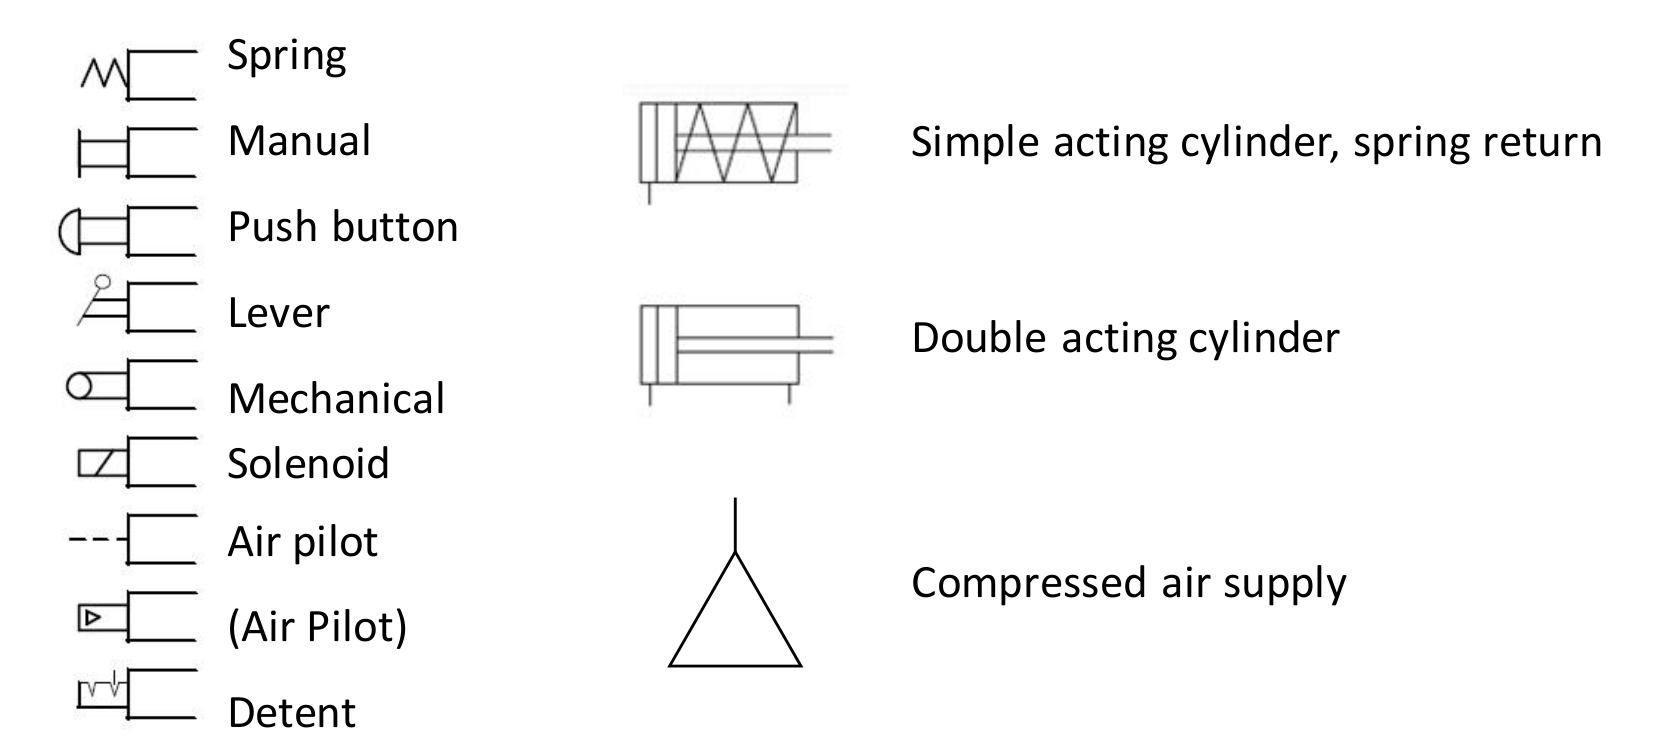
\includegraphics[width=\linewidth]{../../figures/actuation-symbols.png}
\end{center}
{\tiny By José Solis}
\end{frame}
\begin{frame}[label={sec:org3deb9b9}]{Valves}
\begin{center}
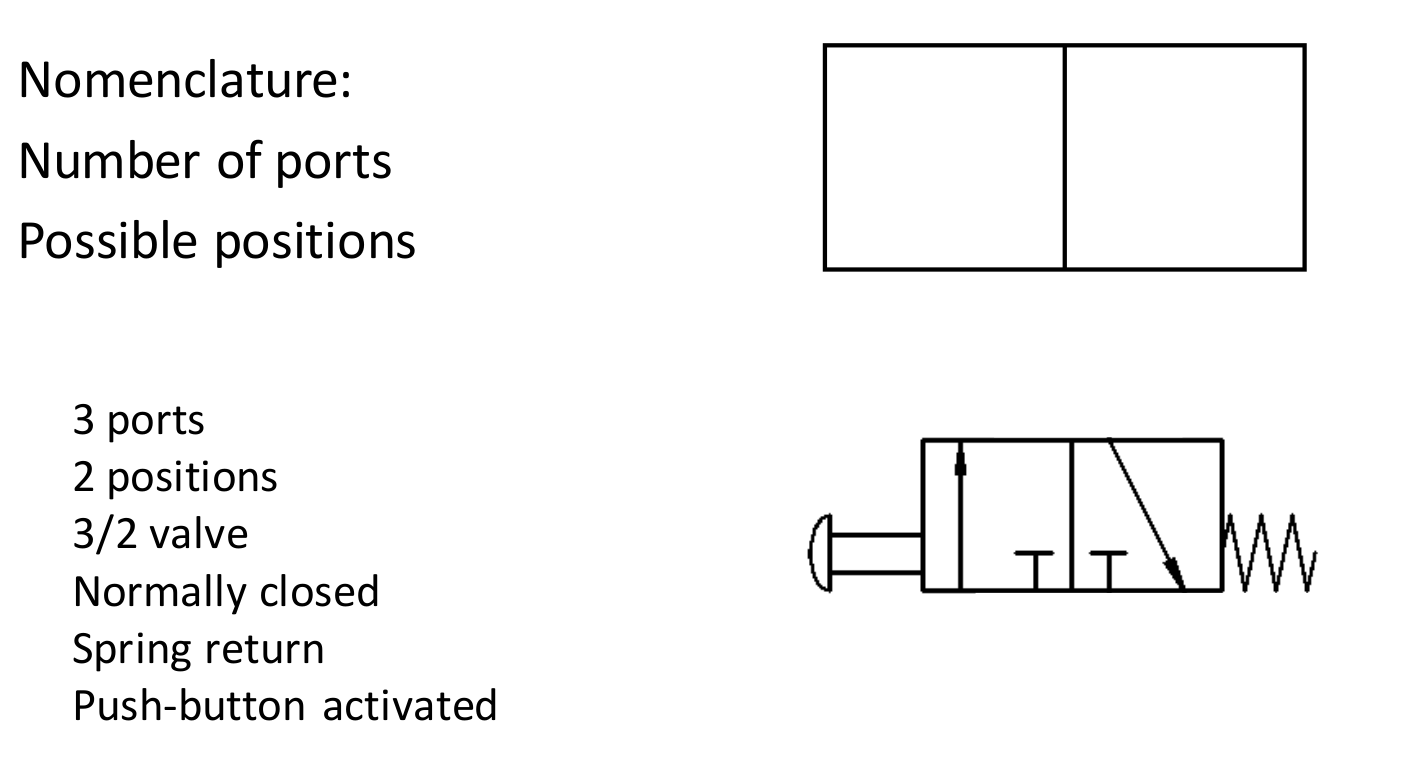
\includegraphics[width=\linewidth]{../../figures/valves-32.png}
\end{center}
{\tiny By José Solis}
\end{frame}
\begin{frame}[label={sec:org015d018}]{Example - 3/2 valve with single acting cylinder}
\begin{center}
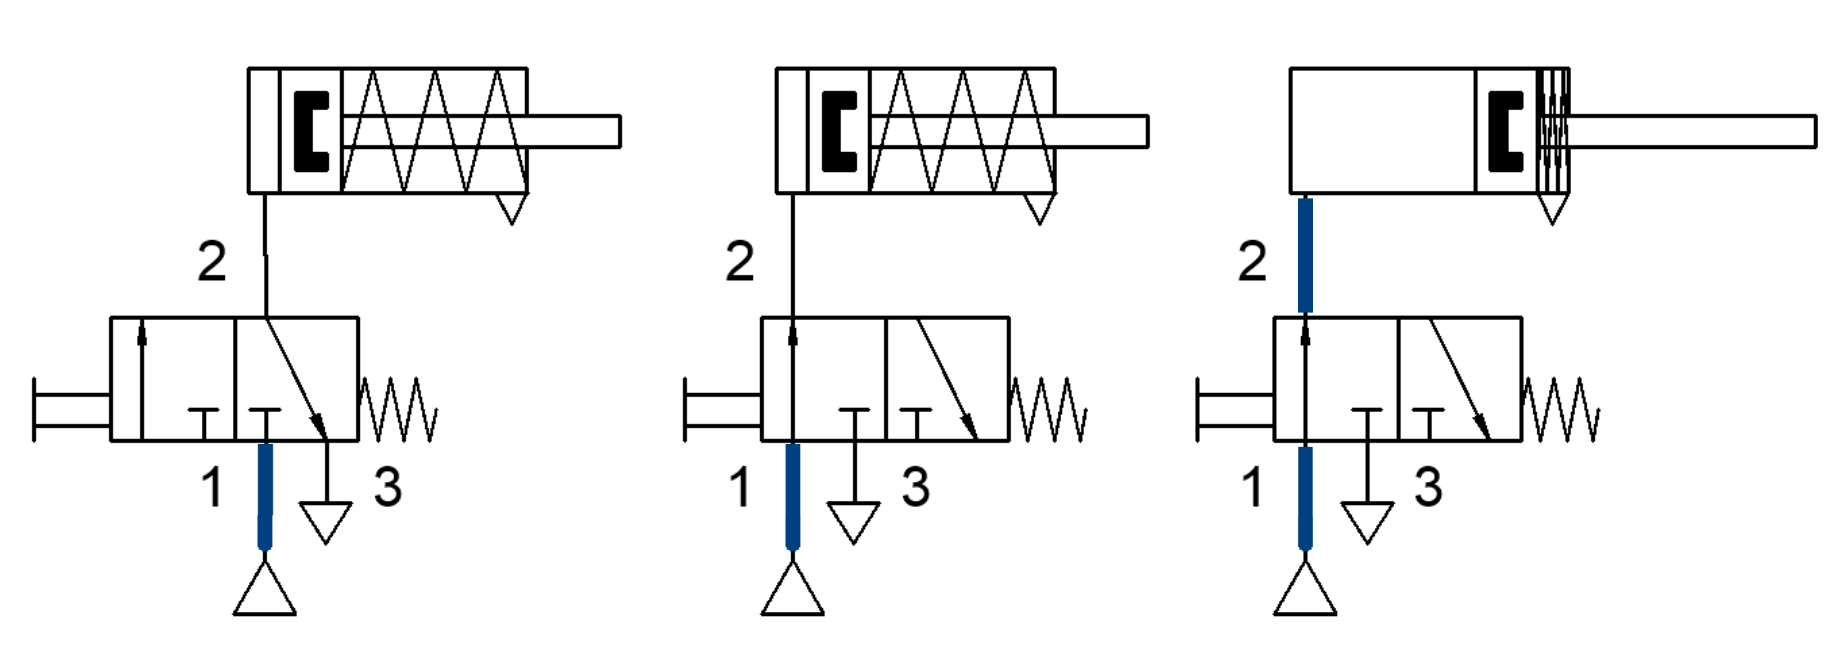
\includegraphics[width=\linewidth]{../../figures/valve-32-example.png}
\end{center}
{\tiny By José Solis}
\end{frame}

\section{Exercise 1 - Single action piston "Stamping"}
\label{sec:orgf0f9c34}
\begin{frame}[label={sec:org9815fc0}]{Exercise - Pressing cheeses}
\begin{center}
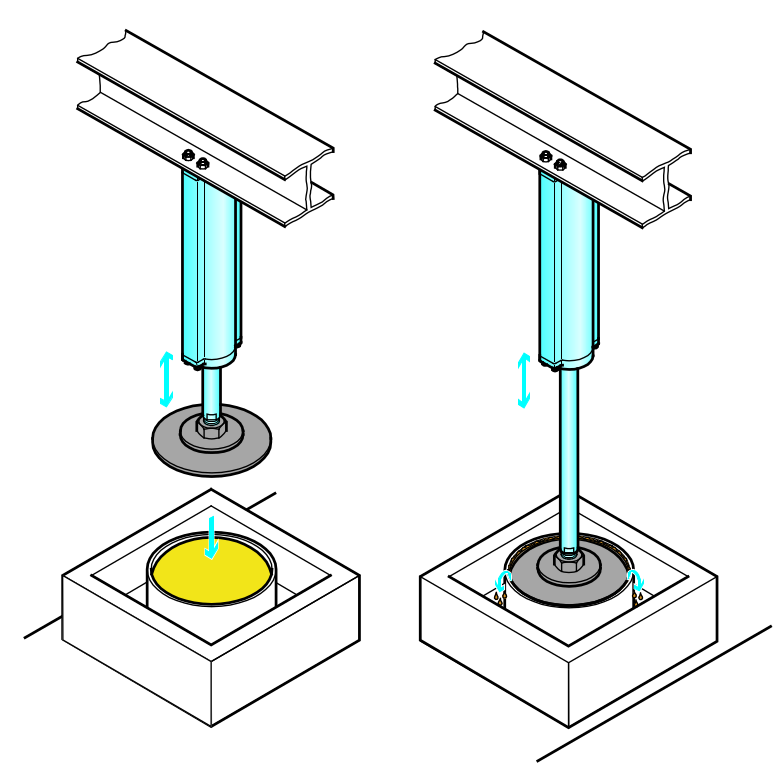
\includegraphics[width=0.4\linewidth]{../../figures/cheese-stamping.png}
\end{center}
{\tiny From FESTO Didactic}
In cheese production a pneumatic cylinder is used to press cheese into a mold. Design and implement a logic control system for this process step.
\end{frame}

\begin{frame}[label={sec:orge2d762c}]{Activity 1 - Explain briefly (individual)}
\begin{center}
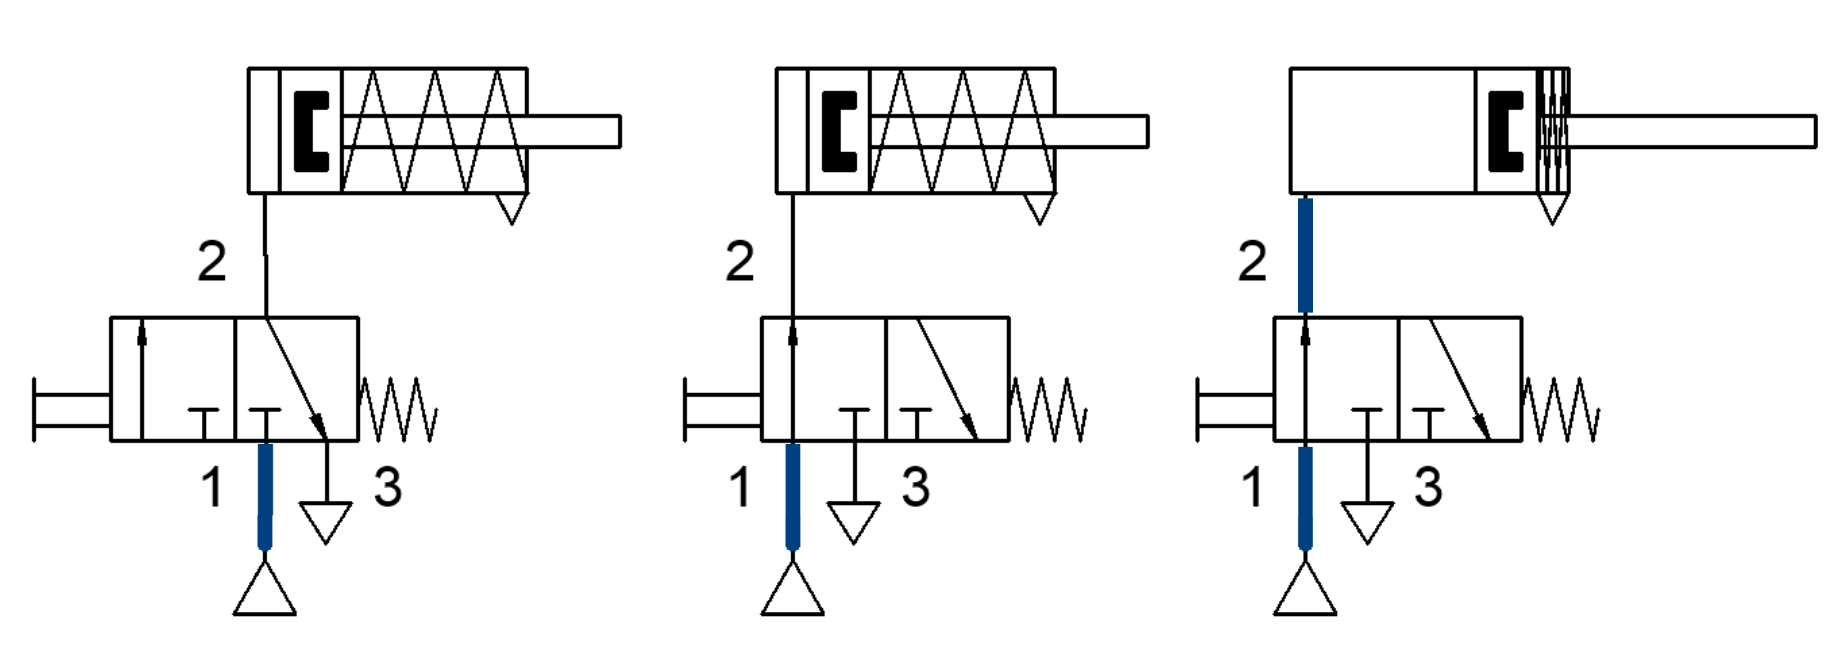
\includegraphics[width=0.5\linewidth]{../../figures/valve-32-example.png}
\end{center}

Answer each question with 2-4 sentences (send in chat directly to prof)

\begin{block}{How does a 3/2 valve work?}
\end{block}
\begin{block}{How does a single-acting cylinder work?}
\end{block}
\end{frame}

\begin{frame}[label={sec:org31b539a}]{Activity 2 - Complete diagram  (group work)}
\begin{columns}
\begin{column}{0.3\columnwidth}
\begin{center}
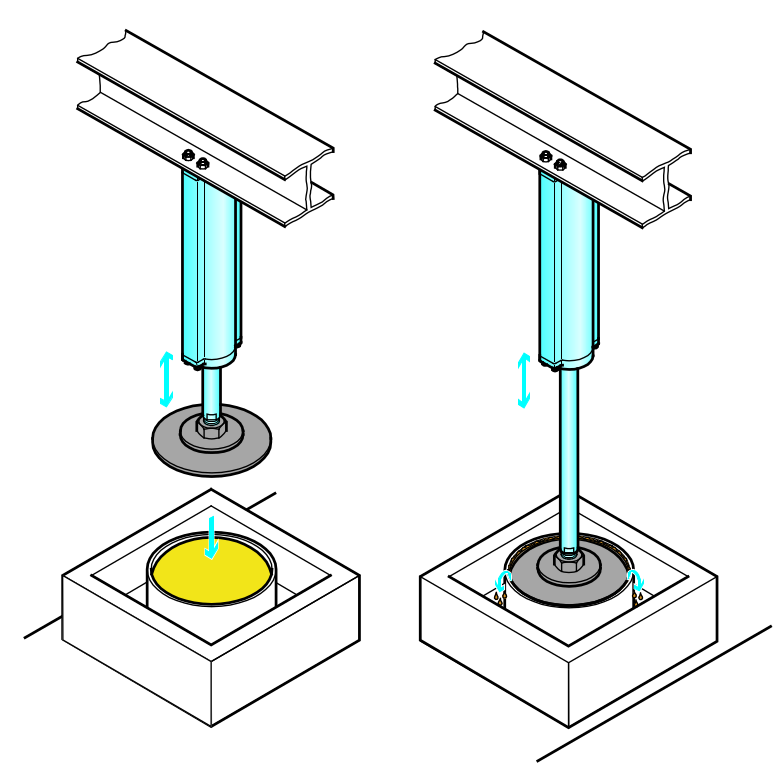
\includegraphics[width=0.8\linewidth]{../../figures/cheese-stamping.png}
\end{center}
{\tiny From FESTO Didactic}
\end{column}
\begin{column}{0.7\columnwidth}
The cylinder should initially be retracted. On the push of a button, it extends. The button causes compressed air to open a 3/2 valve, which in turn directs compressed air to a single-acting cylinder which then extends.  
\end{column}
\end{columns}
\end{frame}

\begin{frame}[label={sec:orgd140bab}]{Activity 2 - Diagram}
\begin{center}
\pgfmathsetmacro\sh{0.3}
\pgfmathsetmacro\cr{.4} % Cylinder radius
\pgfmathsetmacro\cl{2}% Cylinder length
\pgfmathsetmacro\el{0.7*\cr} % Open side of cylinder
\begin{circuitikz}[triangle/.style = {draw, regular polygon, regular polygon sides=3, inner sep=2pt },]

  % Pneumatic circuit
  \node[triangle] (source) at ($ (0,0) + (50mm, -24mm) $) {};
  \node[triangle, left of= source, node distance=5cm] (source2) {};
  \node[above of=source, node distance=3cm] (valve32) {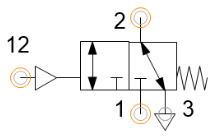
\includegraphics[width=4cm]{../../figures/32-valve-pneum-spring-return-nc.png}};
  \node[draw, minimum width=1cm, minimum height=1cm, left of=valve32, node distance=6cm] (unactivated) {}; 
  \node[draw, minimum width=1cm, minimum height=1cm, right=0mm of unactivated] (activated) {}; 

  \node[coordinate, above of= valve32, node distance=2.9cm] (cylinder) {};
  \draw[thick] (cylinder) -- ++(0, \cr) -- ++ (\cl, 0) -- ++(0, -\el);
  \draw[thick] (cylinder) -- ++(0, -\cr) -- ++ (\cl, 0) -- ++(0, \el);
\end{circuitikz}
\end{center}
\end{frame}

\section{Exercise 2 - Double action piston "Push to extend - push to retract"}
\label{sec:org810d1a1}
\begin{frame}[label={sec:org7c9f1be}]{Double-acting cylinder}
\begin{center}
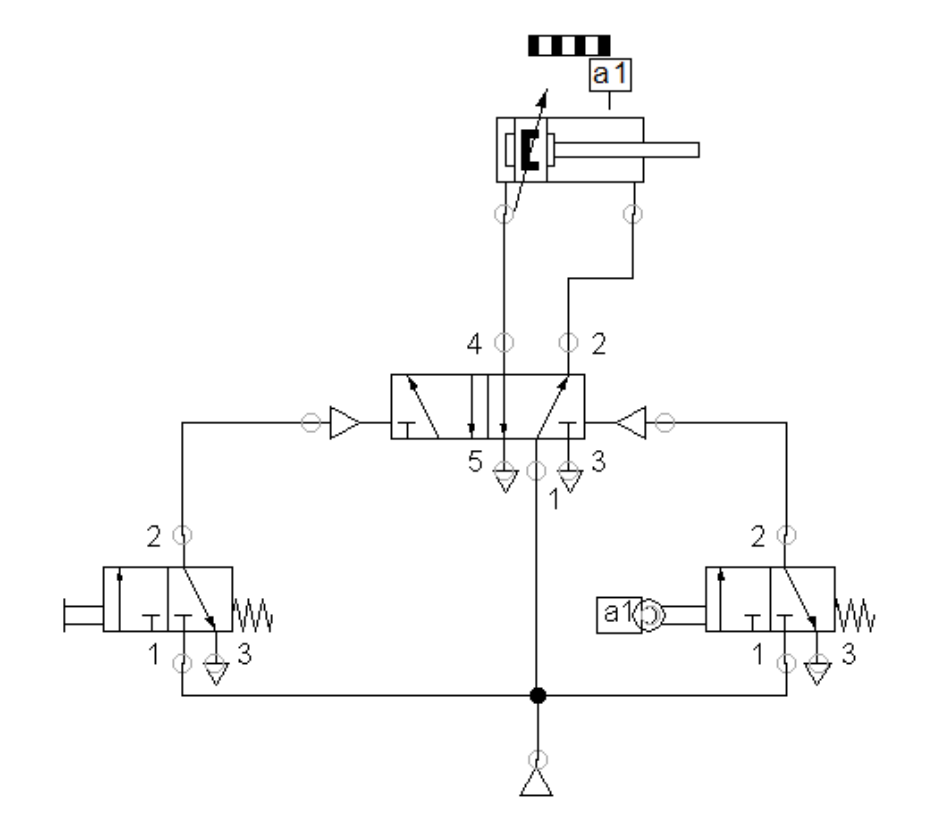
\includegraphics[width=0.7\linewidth]{../../figures/valve-52.png}
\end{center}
\end{frame}
\begin{frame}[label={sec:org2bd930f}]{Double-acting cylinder and the 5/2 valve}
\begin{center}
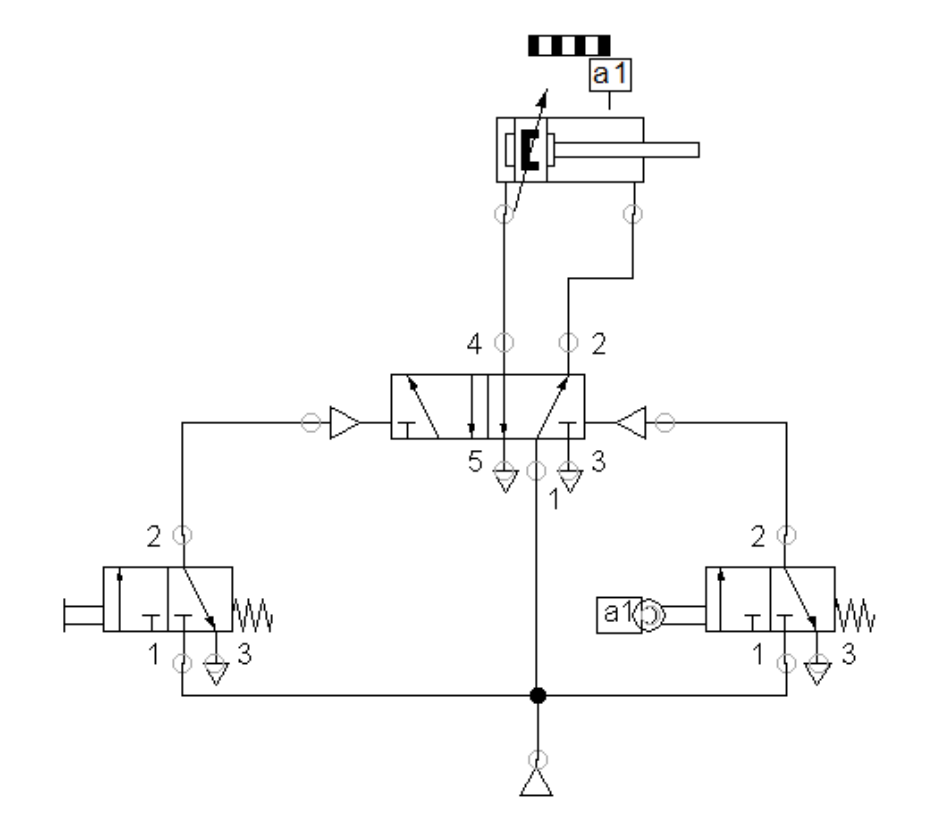
\includegraphics[width=0.7\linewidth]{../../figures/valve-52.png}
\end{center}
\end{frame}


\begin{frame}[label={sec:orgc2cfd6f}]{Activity 3 - Explain briefly (individual)}
Write 2-4 sentences (send in chat directly to prof)
\begin{columns}
\begin{column}{0.4\columnwidth}
\begin{center}
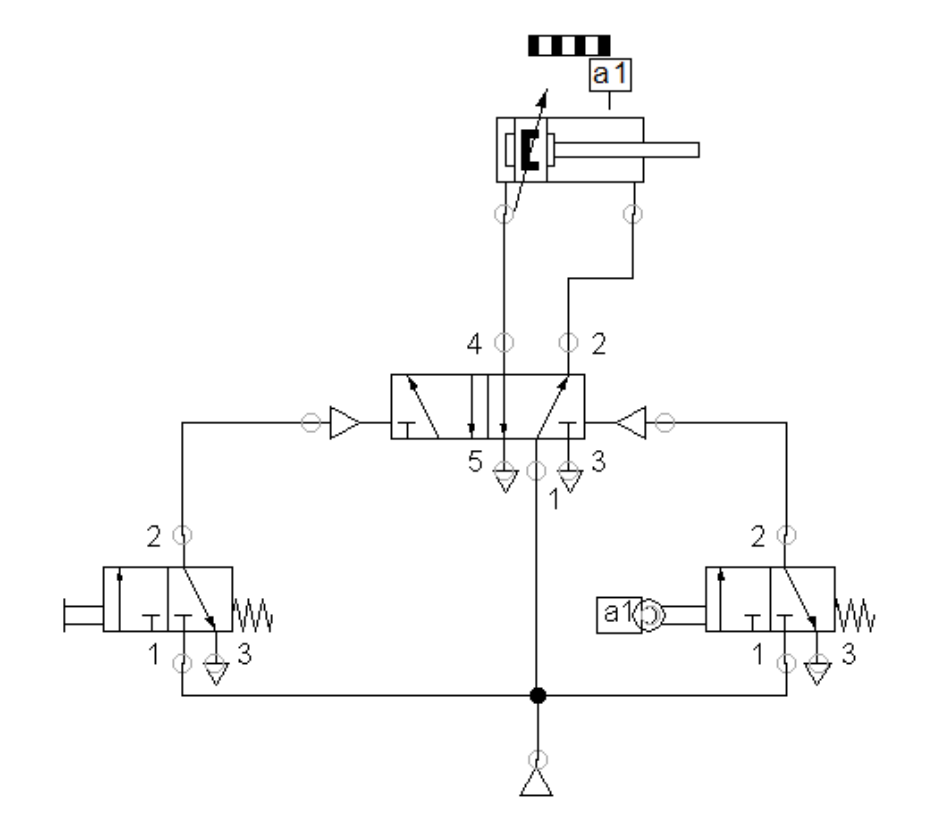
\includegraphics[width=\linewidth]{../../figures/valve-52.png}
\end{center}
\end{column}
\begin{column}{0.6\columnwidth}
\begin{block}{How does a 5/2 valve work?}
\end{block}
\begin{block}{How does a double-acting cylinder work?}
\end{block}
\end{column}
\end{columns}
\end{frame}
\end{document}